\section{Introduction}

\todo[inline]{Why is the subject/problem area important?}
\textit{Wireless sensor networks (WSNs)} have many applications and research studies in areas such as environmental monitoring, agriculture, and military uses (See Table \ref{table:applications}). More recently, the availability and lower cost of low-power wireless transmitters \citep{902661}, solar-harvesting components \citep{Prauzek2018}, and micro-electro-mechanical systems \citep{1045391} has allowed large deployments sizes and scope of use, expanding their real-world use and opening up new areas for practical research \citep{5597912, Kandris2020}.

\todo[inline]{What are the current solutions, what are the problems and how are we improving them?}
WSNs can be structured with centralised, or decentralised control. With centralisation, the controller node has system-wide knowledge, and so allocates measurement tasks to other nodes, orchestrates their communications, and handles recovery. This approach inherently does not scale to large networks due to congestion and resource exhaustion on the central component. In harsh environments, this centralisation of control is not robust to damage or node loss. For these reasons, we focus on decentralised, autonomous methods for WSN construction.

With decentralisation, nodes have a localised knowledge only, and autonomously orchestrate the same functionality, sometimes being organised into groups to increase co-ordination without full centralisation. This ability for nodes to work autonomously increases resilience. However, we now have problems in working from local information and coordination of actions across the systems nodes. Broadly there are three main categories for decentralisation \citep{10.1007/978-3-642-11814-2_4, 10.1504/IJCNDS.2012.048871},
\begin{itemize}
	\item \textit{Clustering}
	\item \textit{Hierarchical}
	\item \textit{Reinforcement learning}
\end{itemize}
\todo[inline]{Integrate the hiearchical diagram and add clustering example}
\begin{figure}[]
	\centering
	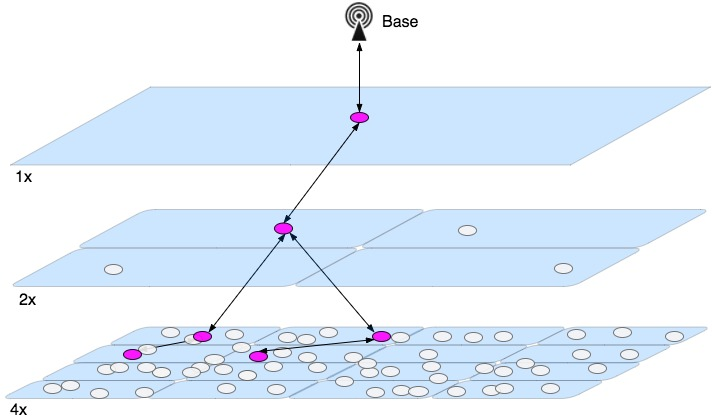
\includegraphics[width=0.5\linewidth]{WSN_hierarchical_resolution}
	\caption{Agent system hierarchical neighbourhood resolution: shows one of the possible modes of hierarchical networking that can be formed by the agent system through per-agent local neighbourhood learning. The initial agent passes requests through smaller and smaller neighbourhoods until the granulaity of the data meets that of the request}
	\label{fig:wsnhierarchicalresolution}
\end{figure}
\todo[inline]{What is the solution and contributions we present?}
The solution we present here is based on the following algorithms previously developed by the authors. We use the \acronymATARIA{}{} algorithm to optimise the task of measurements and coverage, minimise the energy consumption of the network, while adapting to the dynamic nature of WSNs \citep{creech2021dynamic}. Through the \acronymMGRAO{}{} algorithm we enable sensors that are taking measurements to optimise the allocation of their resources to meet the overall system goal \citep{creech2021resource}. By combining and evaluating these algorithms in a simulated WSN deployed in a realistic environment, we show that the overall solution can be successfully utilised to balance the systems' multiple objectives of minimising energy consumption, maximising system lifetime, as well as optimising the quality of the measurement tasks while still maintaining geographical coverage.
\todo[inline]{Structure of paper}
In Section \ref{section:background} we look at related research in this area, allowing us to concretely define the problem in Section \ref{section:problem}. Section \ref{section:solution} sets out our solution, followed by definition of the simulated environment and evaluation of the solution in Section \ref{section:experimental}. We close with the summary of our conclusions and future work in Section \ref{section:conclusions}.


\begin{table}
	\footnotesize
	\begin{tabular}{|p{0.2\textwidth}|p{0.2\textwidth}|p{0.5\textwidth}|}
		\hline
		Area & References & Summary \\
		\hline
		Ocean monitoring and the marine environment & \cite{Mahdy2008a, Albaladejo2010, 6973877} & XXX \\
		Radiation contamination & \cite{Gomez2015} & XXX \\
		Water quality & \cite{Fang2010} & XXX \\
		Agriculture  & \cite{8745854} & XXX \\
		Volcano monitoring  & \cite{Werner-Allen2006} & XXX \\
		Flood monitoring  & \cite{Castillo-effen2004} & XXX \\
		Military & \cite{6268958} & XXX \\
		\hline
	\end{tabular}
	\caption{Real-world applications of wireless sensor networks}
	\label{table:applications}	
\end{table}
